\documentclass[aspectratio=169,11pt,hyperref={colorlinks=true}]{beamer}
\usetheme{boxes}
\setbeamertemplate{navigation symbols}{}
\definecolor{openstack}{RGB}{149,0,4}
\setbeamercolor{titlelike}{fg=openstack}
\setbeamercolor{structure}{fg=openstack}
\hypersetup{colorlinks,urlcolor=openstack}
\setbeamertemplate{footline}[frame number]
% Inserting graphics
\usepackage{graphicx}
% Side-by-side figures, etc
\usepackage{subfigure}
% Code snippits
\usepackage{listings}
% Color stuff
\usepackage{color}
\usepackage{amsmath}
\usepackage{tikz}
\newcommand\RBox[1]{%
  \tikz\node[draw,rounded corners,align=center,] {#1};%
}
\usepackage{hyperref}
%\usecolortheme{buzz}
%\usecolortheme{wolverine}
%\usetheme{Boadilla}
\usepackage[T1]{fontenc}

\definecolor{mygreen}{rgb}{0,0.6,0}
\definecolor{mygray}{rgb}{0.5,0.5,0.5}
\definecolor{mymauve}{rgb}{0.58,0,0.82}

\lstset{%
  backgroundcolor=\color{white},   % choose the background color; you must add \usepackage{color} or \usepackage{xcolor}
  breakatwhitespace=false,         % sets if automatic breaks should only happen at whitespace
  breaklines=true,                 % sets automatic line breaking
  captionpos=b,                    % sets the caption-position to bottom
  commentstyle=\color{openstack},  % comment style
  extendedchars=true,              % lets you use non-ASCII characters; for 8-bits encodings only, does not work with UTF-8
  keepspaces=true,                 % keeps spaces in text, useful for keeping indentation of code (possibly needs columns=flexible)
  keywordstyle=\color{blue},       % keyword style
%  otherkeywords={*,...},           % if you want to add more keywords to the set
  numbersep=5pt,                   % how far the line-numbers are from the code
  numberstyle=\tiny\color{mygray}, % the style that is used for the line-numbers
  rulecolor=\color{black},         % if not set, the frame-color may be changed on line-breaks within not-black text (e.g. comments (green here))
  showspaces=false,                % show spaces everywhere adding particular underscores; it overrides 'showstringspaces'
  showstringspaces=false,          % underline spaces within strings only
  showtabs=false,                  % show tabs within strings adding particular underscores
  stringstyle=\color{openstack},   % string literal style
}

\setbeamerfont{caption}{series=\normalfont,size=\fontsize{6}{8}}
\setbeamertemplate{caption}{\raggedright\insertcaption\par}

\setlength{\abovecaptionskip}{0pt}
\setlength{\floatsep}{0pt}

\author[Matthew Treinish]{%
    \texorpdfstring{%
        \centering
        Matthew Treinish\\
        \href{mailto:mtreinish@kortar.org}{mtreinish@kortar.org}\\
        \texttt{mtreinish on Freenode}\\
        \href{https://github.com/mtreinish/building-a-better-thermostat}{https://github.com/mtreinish/building-a-better-thermostat}
   }
   {Matthew Treinish}
}
\date{March 18, 2017}

\title{Building a Better Thermostat}
\begin{document}

%{%
%\setbeamertemplate{footline}{}
%\begin{frame}[noframenumbering]
%    \setbeamercolor{titlelike}{fg=white}
%    \setbeamercolor{structure}{fg=white}
%    \setbeamercolor{normal text}{fg=white}
%    \hypersetup{colorlinks,urlcolor=white}
%    \setbeamercolor{author}{fg=white}
%    \setbeamercolor{date}{fg=white}
%    \setbeamercolor{background}{bg=openstack}
%    \titlepage{}
%    \centering
%    \href{https://github.com/mtreinish/building-a-better-thermostat}{https://github.com/mtreinish/building-a-better-thermostat}
%\end{frame}
%}
\titlepage

\section{My Apartment}
\begin{frame}
    \frametitle{Room Layout}
    \begin{center}
    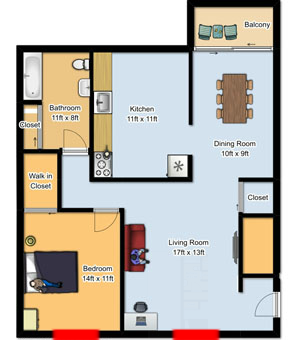
\includegraphics[height=.85\textheight]{floorplan.png}
    \end{center}
\end{frame}

\begin{frame}
    \frametitle{AC Units}
    \begin{center}
        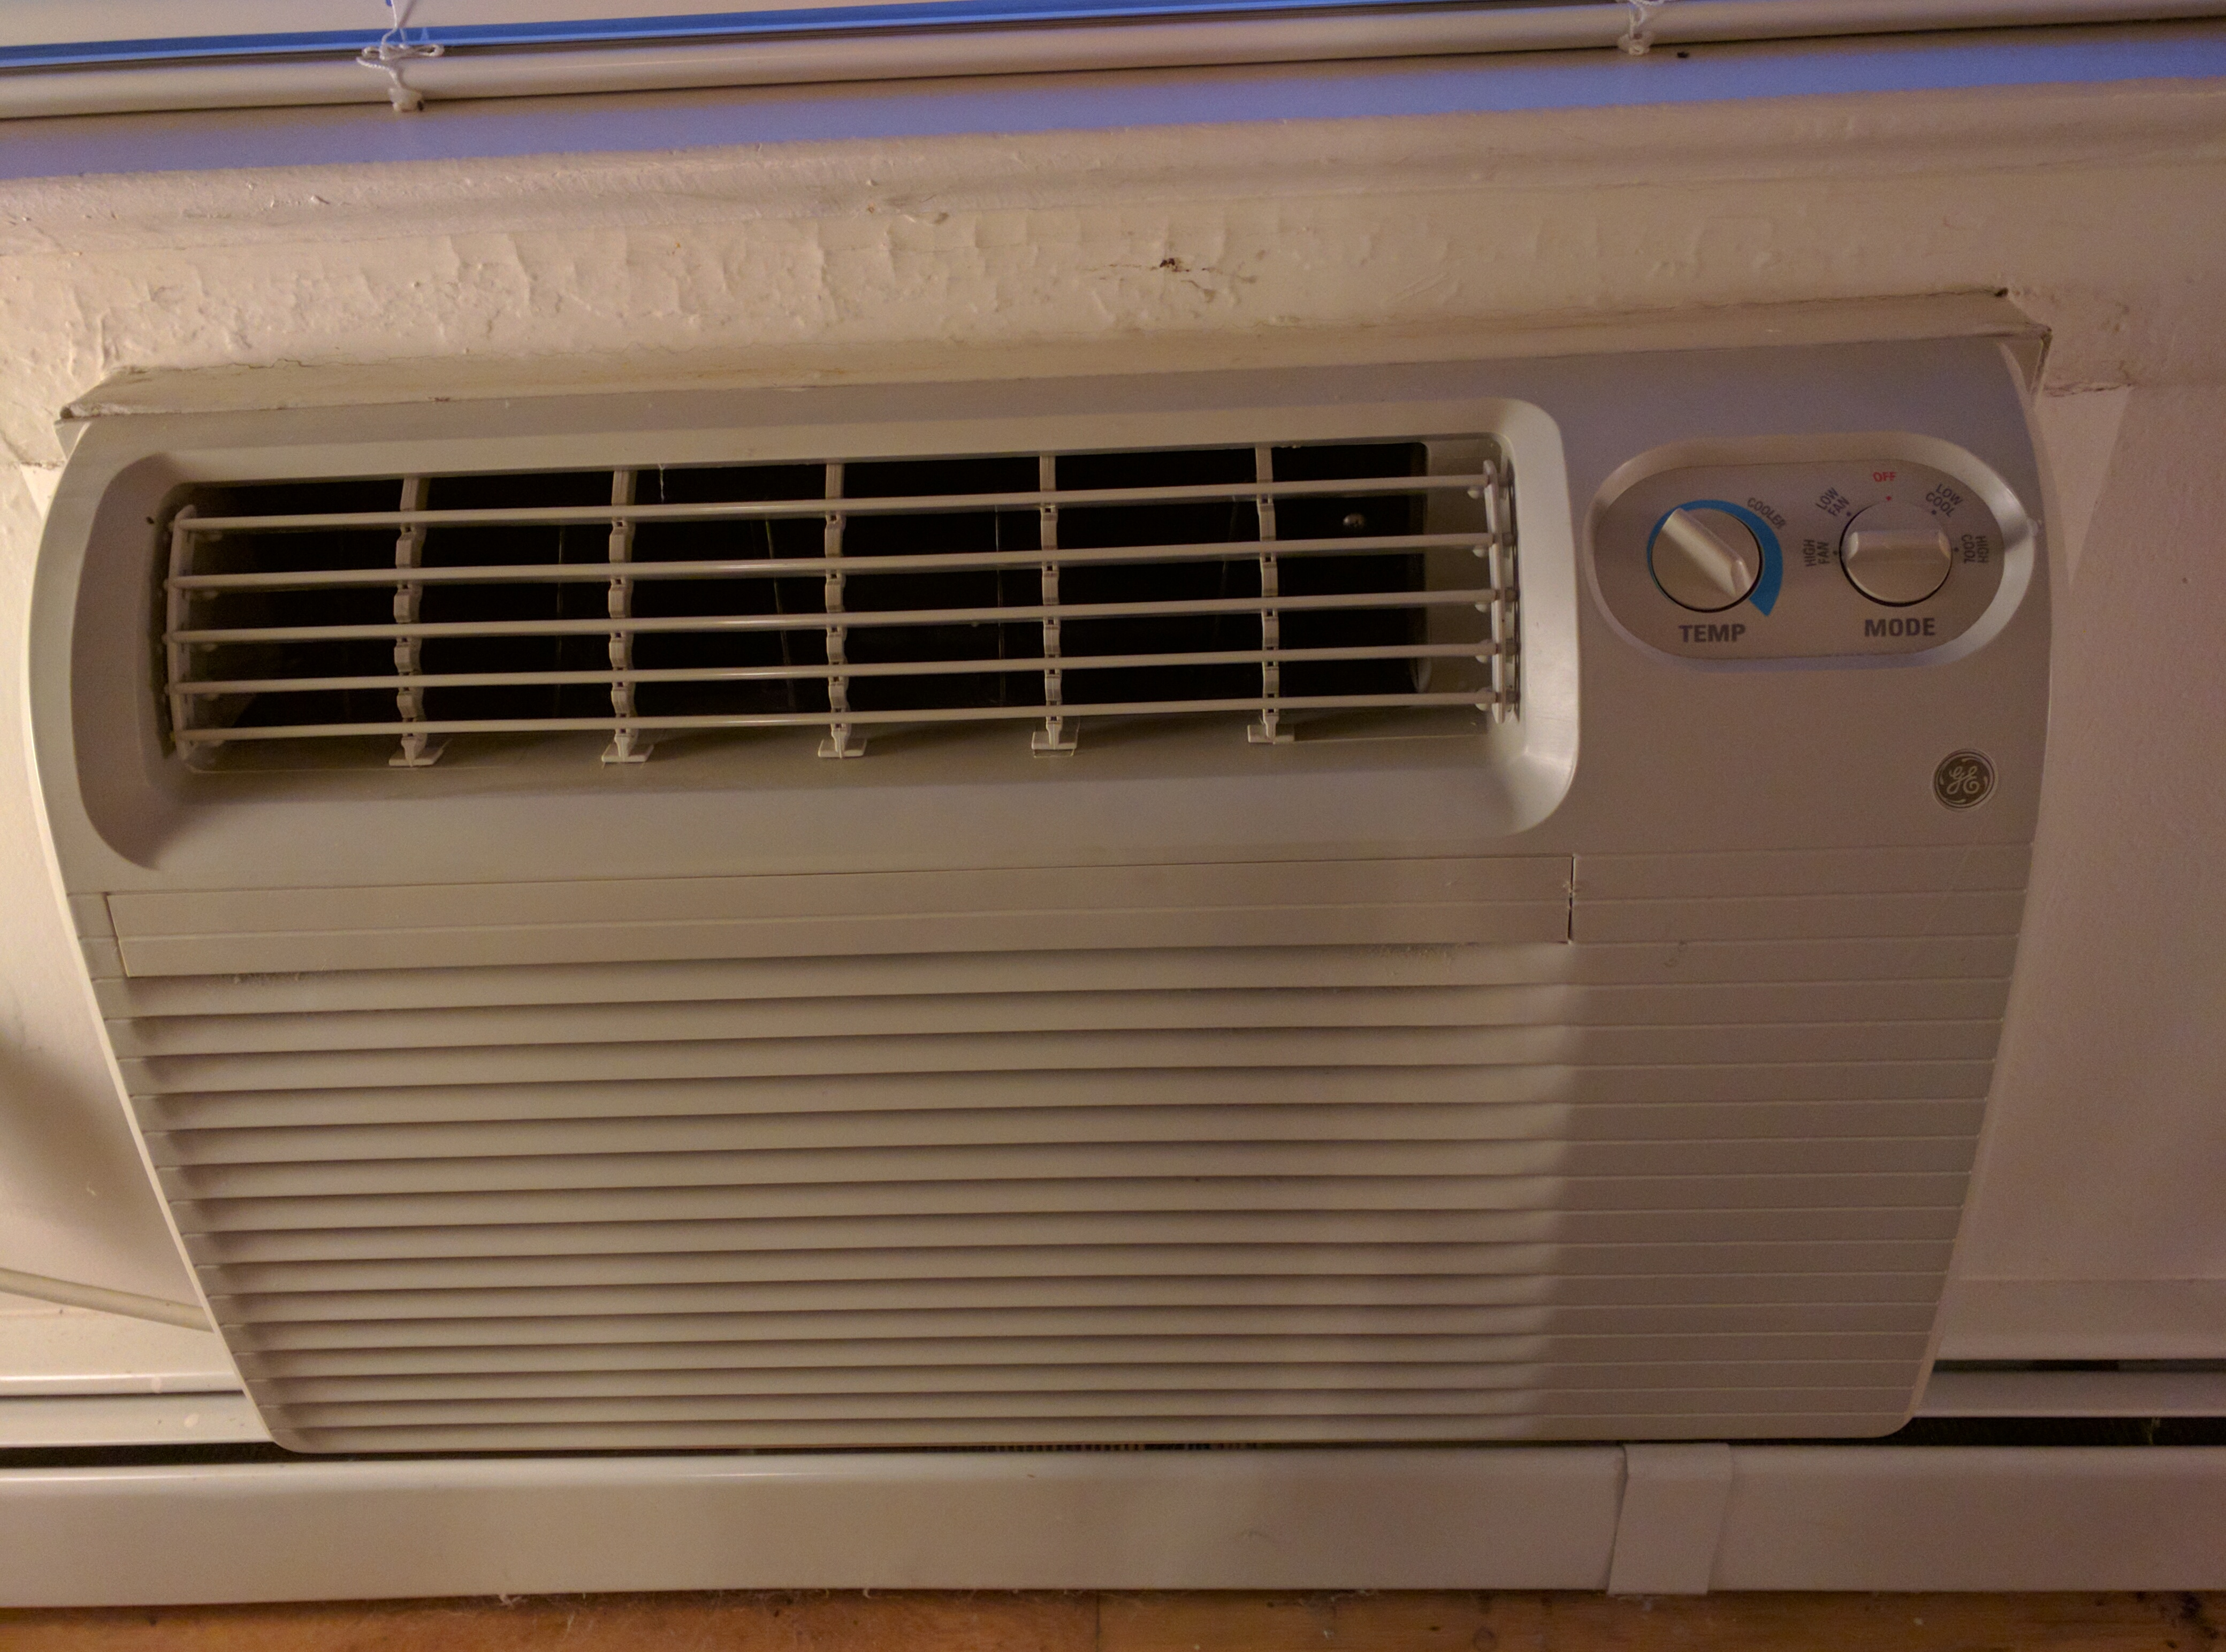
\includegraphics[width=.75\textwidth]{AC_unit.jpeg}
    \end{center}
\end{frame}

\section{Builing a Thermostat}

\begin{frame}
    \frametitle{Thermostat}
    \begin{itemize}
        \item Closed Loop control device
        \item 1 input temperature sensor
        \item 1 output for controlling heating and/or cooling system
    \end{itemize}
\end{frame}

\subsection{Living Room Hardware}
\begin{frame}
    \frametitle{Controlling the AC}
    \begin{itemize}
        \item Can't take apart the AC (I don't own it)
        \item No identifying information for the AC
        \item Control via power (use a relay to turn on and off)
    \end{itemize}
\end{frame}

\begin{frame}
    \begin{columns}[T]
        \begin{column}{.48\textwidth}
            \begin{itemize}
                \item Use Z-Wave outlet to control
                \item
            \end{itemize}
        \end{column}
        \begin{column}{.48\textwidth}       
            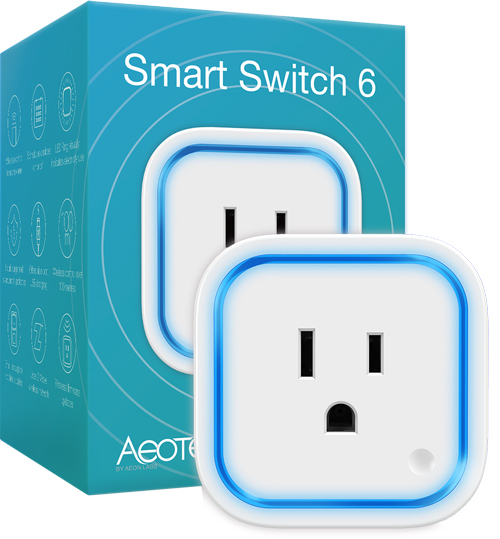
\includegraphics[width=.8\textwidth]{aeotec-ss6.jpg}
        \end{column}
    \end{columns}
\end{frame}

\begin{frame}
    \frametitle{Sensing the Living Room Temperature}
    \begin{itemize}
        \item Wireless sensor 
        \item Leverage Z-Wave network
        \item 
    \end{itemize}
\end{frame}

\subsection{Bedroom Temperature Sensing}
\begin{frame}
    \frametitle{Bedroom Temperature Sensing}
    \begin{columns}[T]
        \begin{column}{.48\textwidth}
            \begin{itemize}
                \item Track both bedroom and ``data`` closet temperatures
                \item Leverage spare raspberry pi sitting in ``data'' closet
                \item Went with dallas 1 wire temperature sensors
            \end{itemize}
        \end{column}
        \begin{column}{.48\textwidth}
            \centering
            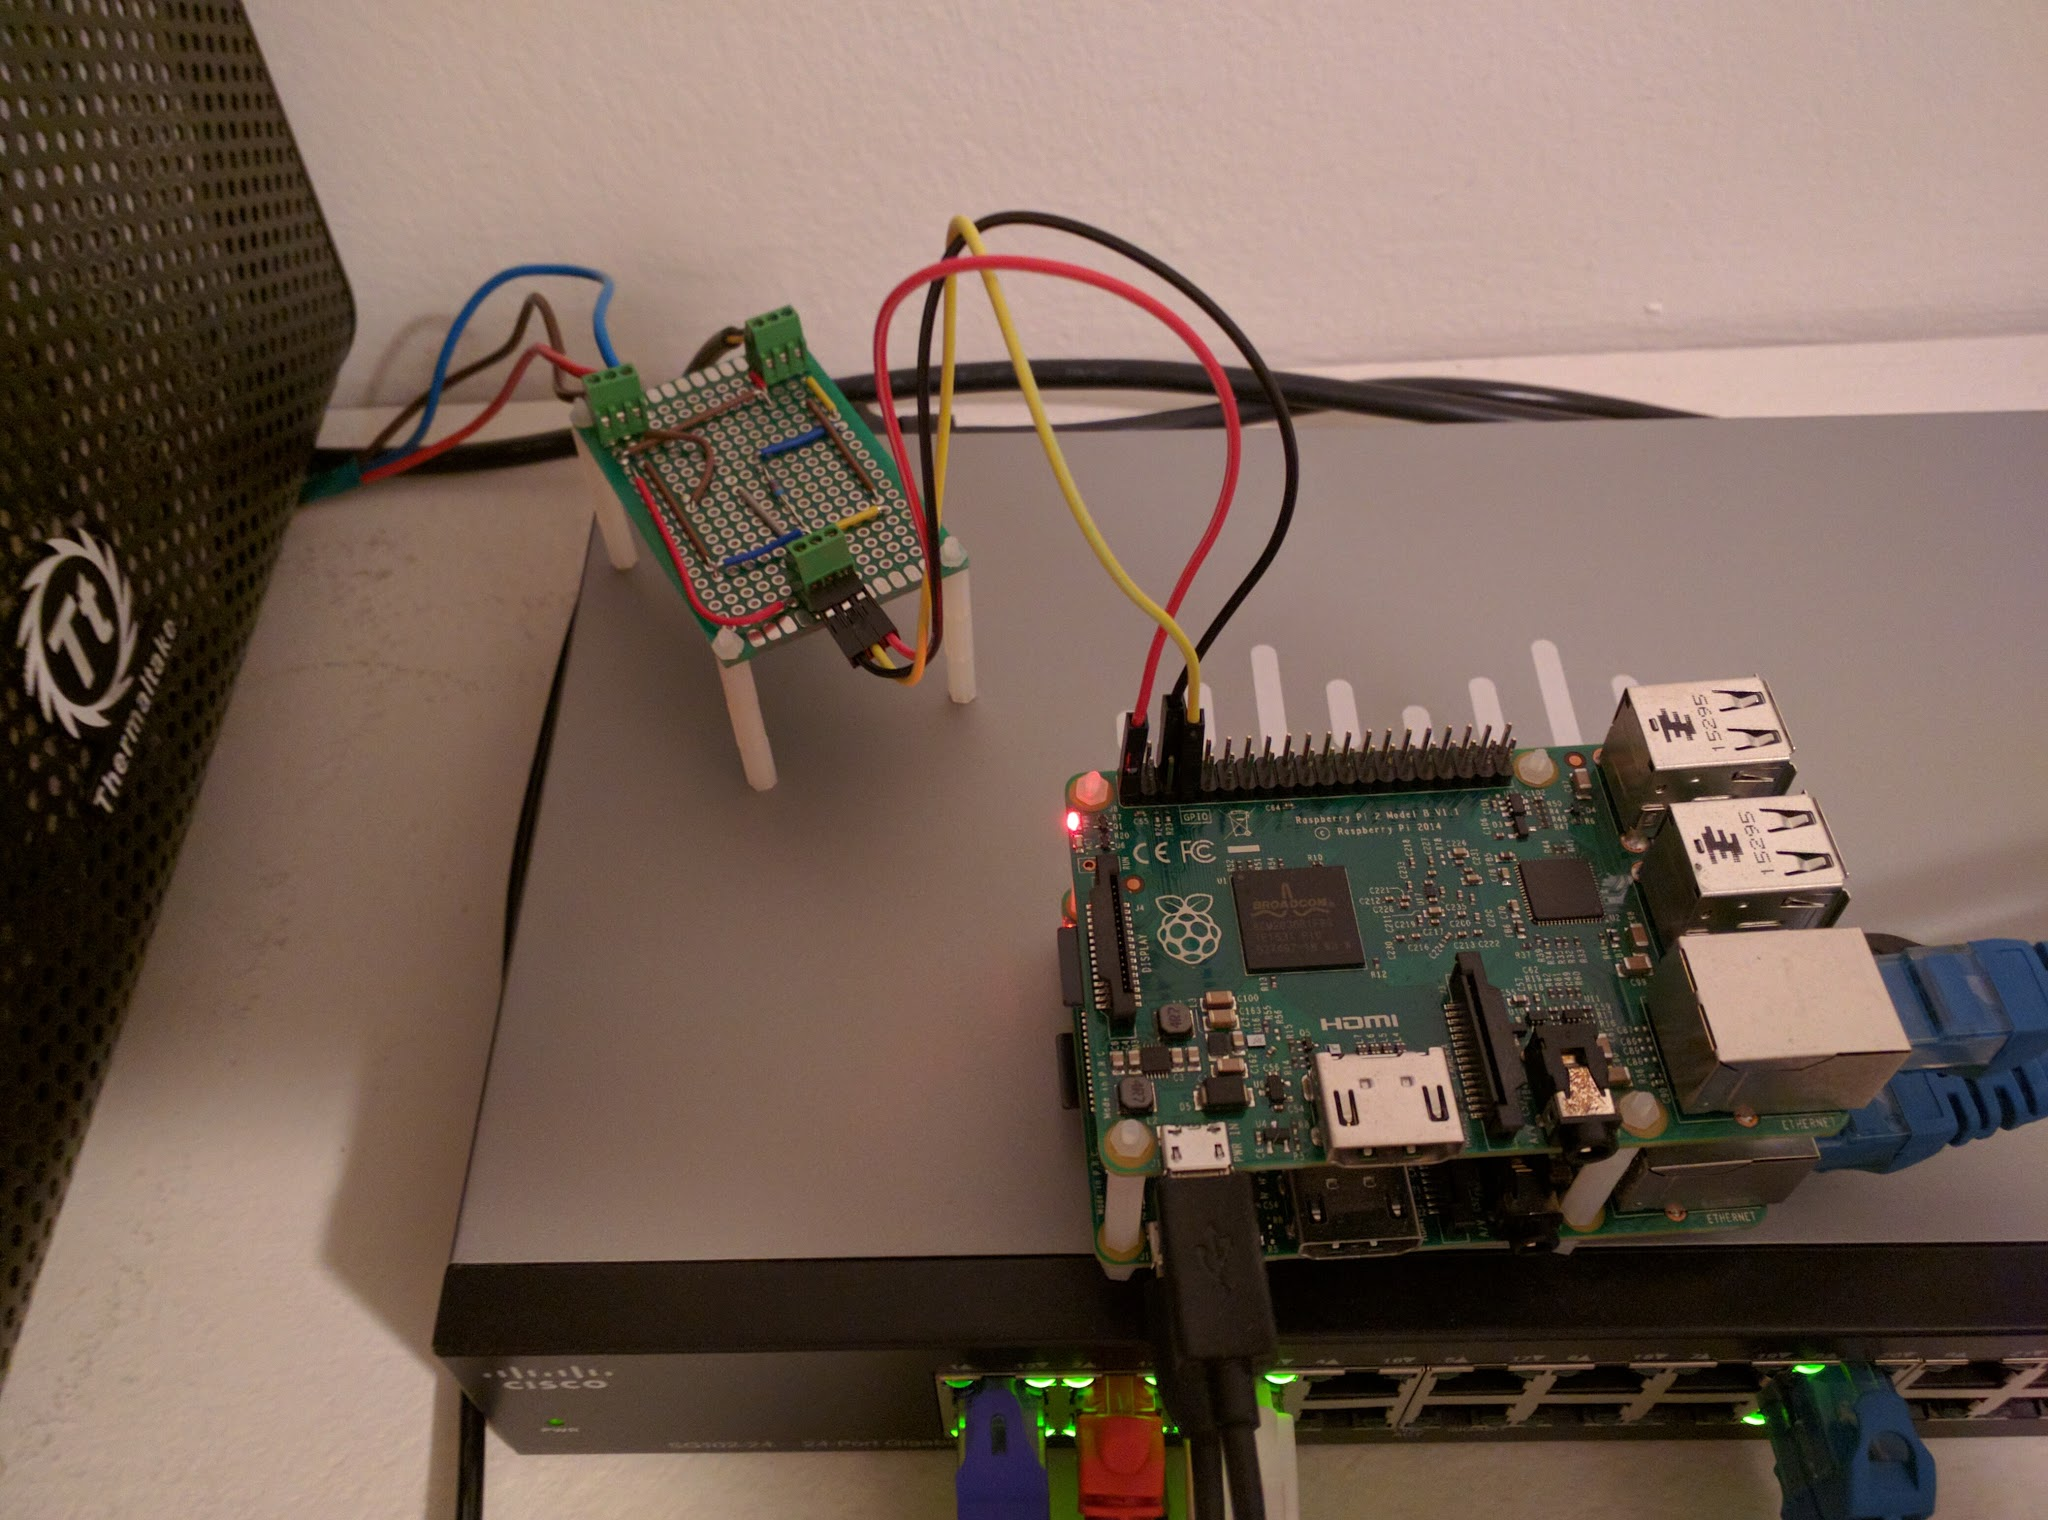
\includegraphics[width=\textwidth]{raspi.jpg}
        \end{column}
    \end{columns}
\end{frame}

\subsection{Software}
\begin{frame}
    \frametitle{Home Assistant}
    \begin{itemize}
        \item Open Source Home Automation Platform
        \item Written in Python 3
        \item Has support for over 600 different components
        \item Runs locally (with all data locally)
    \end{itemize}
\end{frame}

\begin{frame}
    \frametitle{Setting up thermostat in Home Assistant}
    \begin{columns}[T]
        \begin{column}{.48\textwidth}
%            \href{https://home-assistant.io/components/#climate}{https://home-assistant.io/components/#climate}
            \centering
            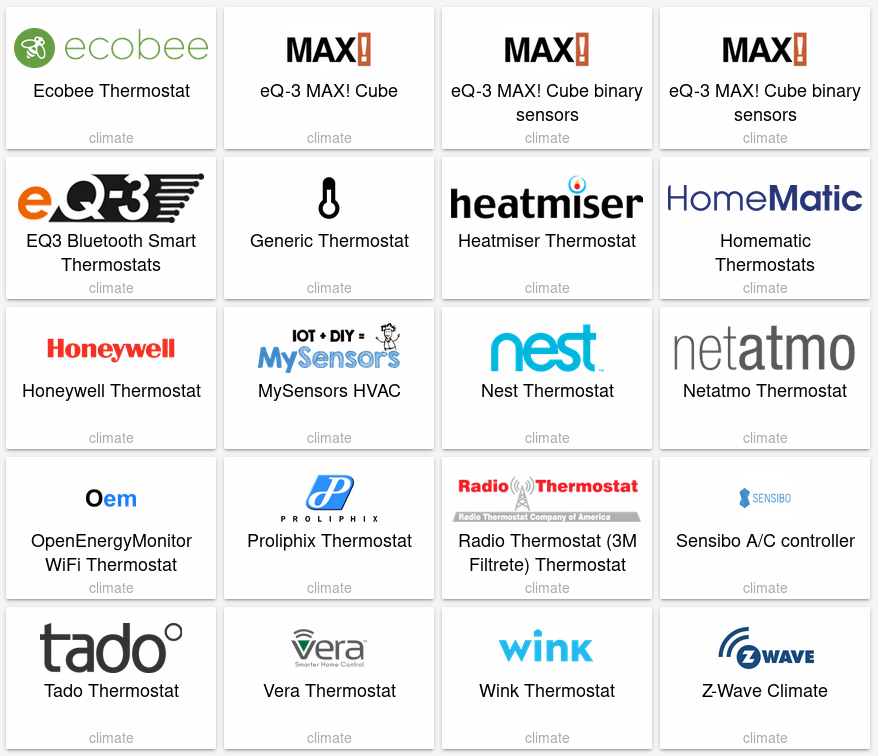
\includegraphics[width=\textwidth]{thermostat_components.png}
        \end{column}
        \begin{column}{.48\textwidth}
            \begin{itemize}
                \item Use the generic thermostat component
            \end{itemize}
        \end{column}
    \end{columns}
\end{frame}

\begin{frame}
    \begin{center}
        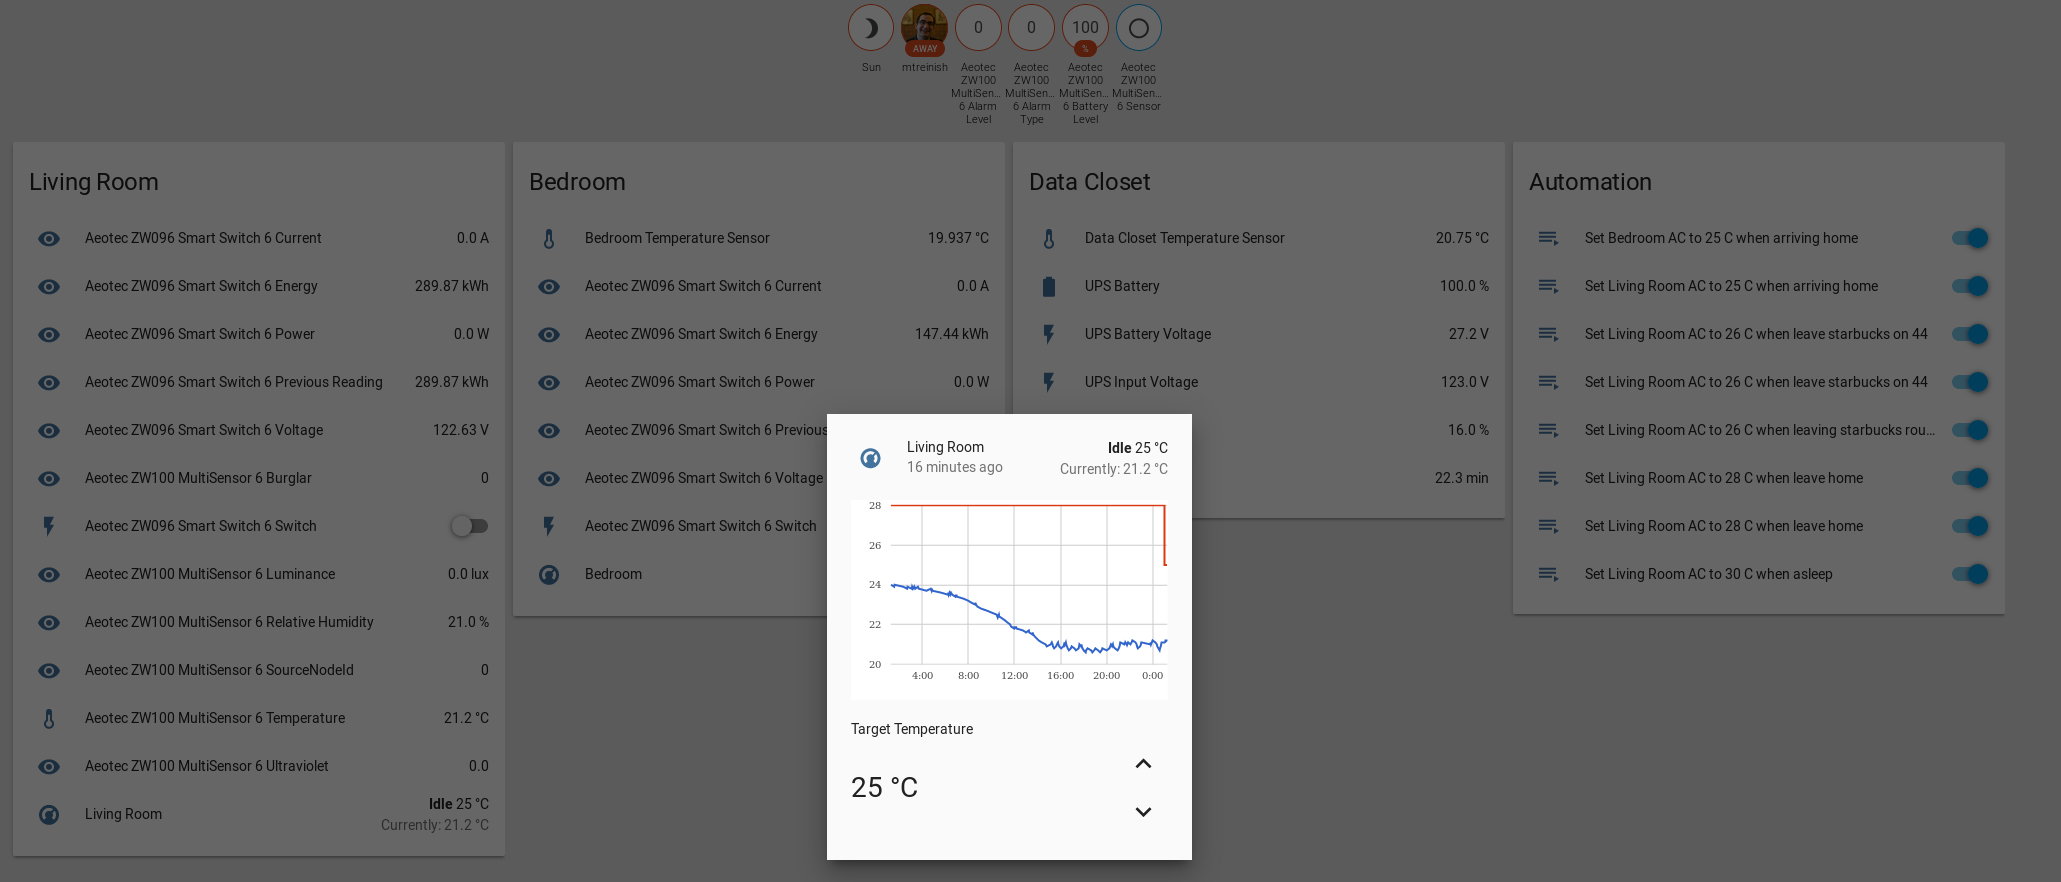
\includegraphics[width=\textwidth]{Control_panel.png}
    \end{center}
\end{frame}

\begin{frame}
    \frametitle{DallasMQTT}
    \begin{itemize}
        \item Framework for polling sensors and pushing results on MQTT
        \item Handles an arbitrary number of sensors
        \item Currently only supports Dallas 1 wire temperature sensors from w1\_therm linux driver
        \item Written in python
    \end{itemize}
\end{frame}

\section{Initial Issues}

\begin{frame}
    \frametitle{Short Cycle Time}
    \begin{center}
        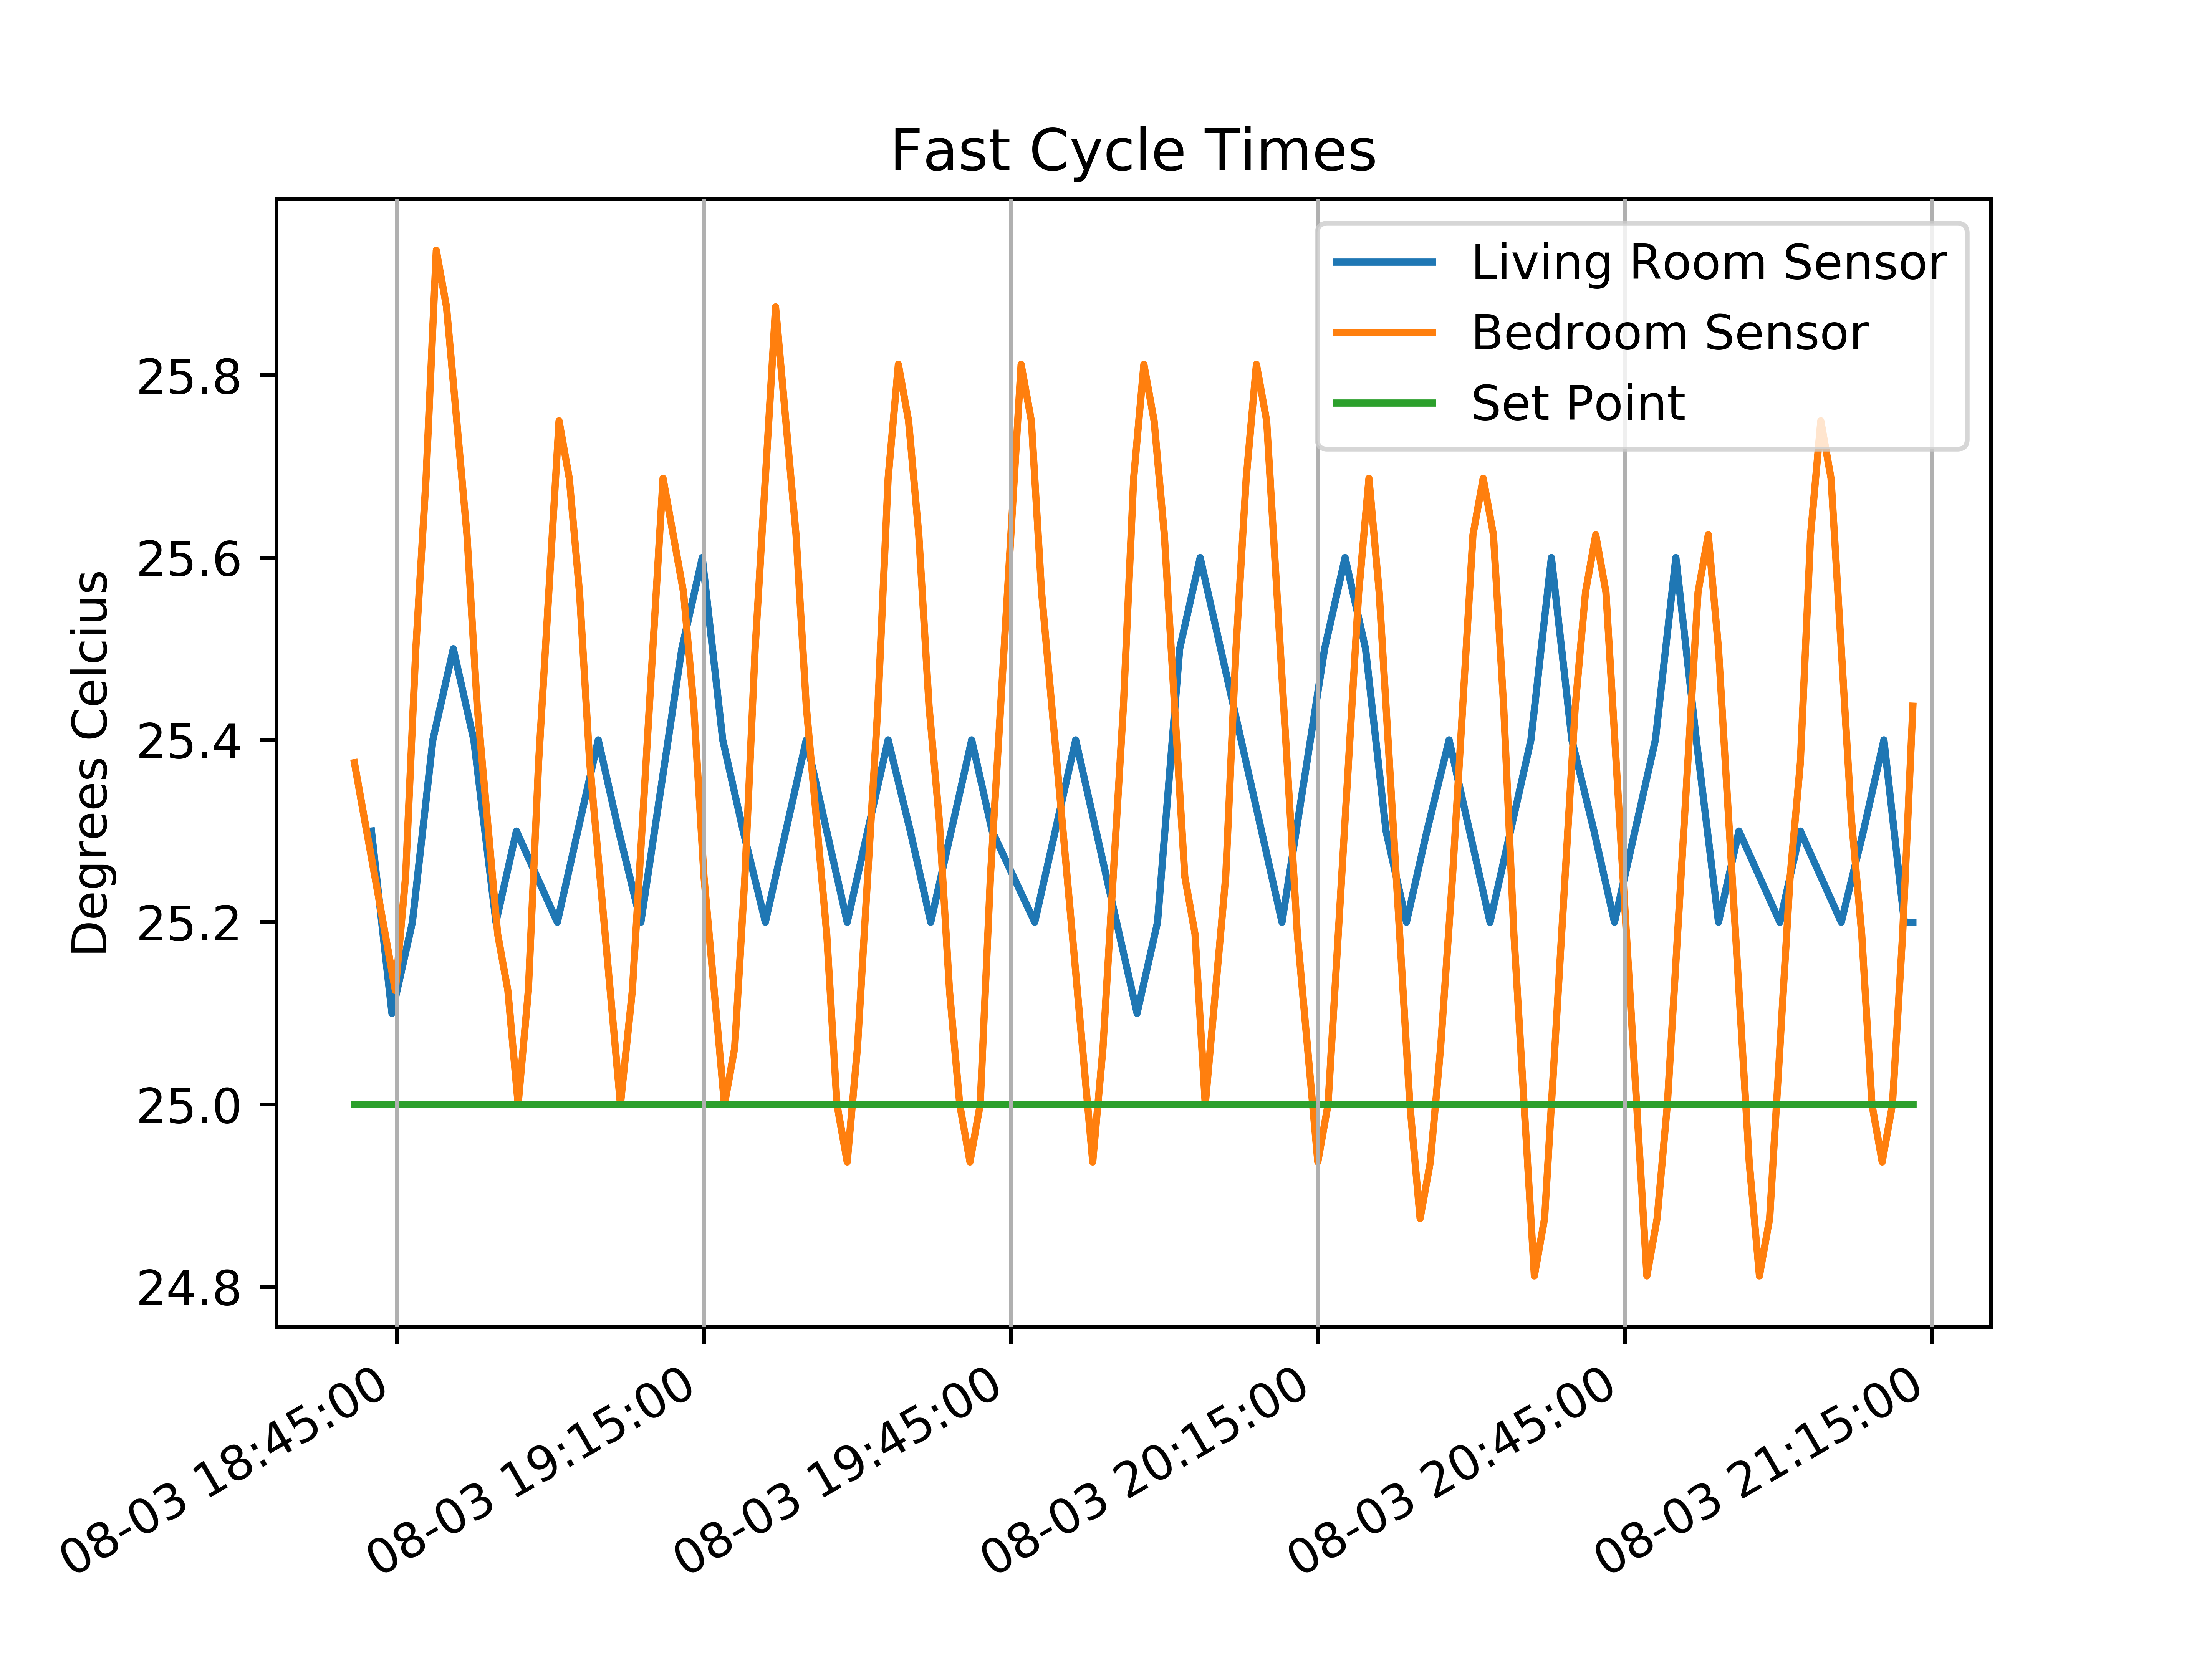
\includegraphics[height=.75\textheight]{short_cycle.png}
    \end{center}
    \begin{itemize}
        \item Bedroom on for 8 min. and off for 4 min.
        \item Living Room on for 4 min. off for 2 min.
    \end{itemize}
\end{frame}

\begin{frame}
    \frametitle{Corrected Cycle Time}
    \begin{center}
        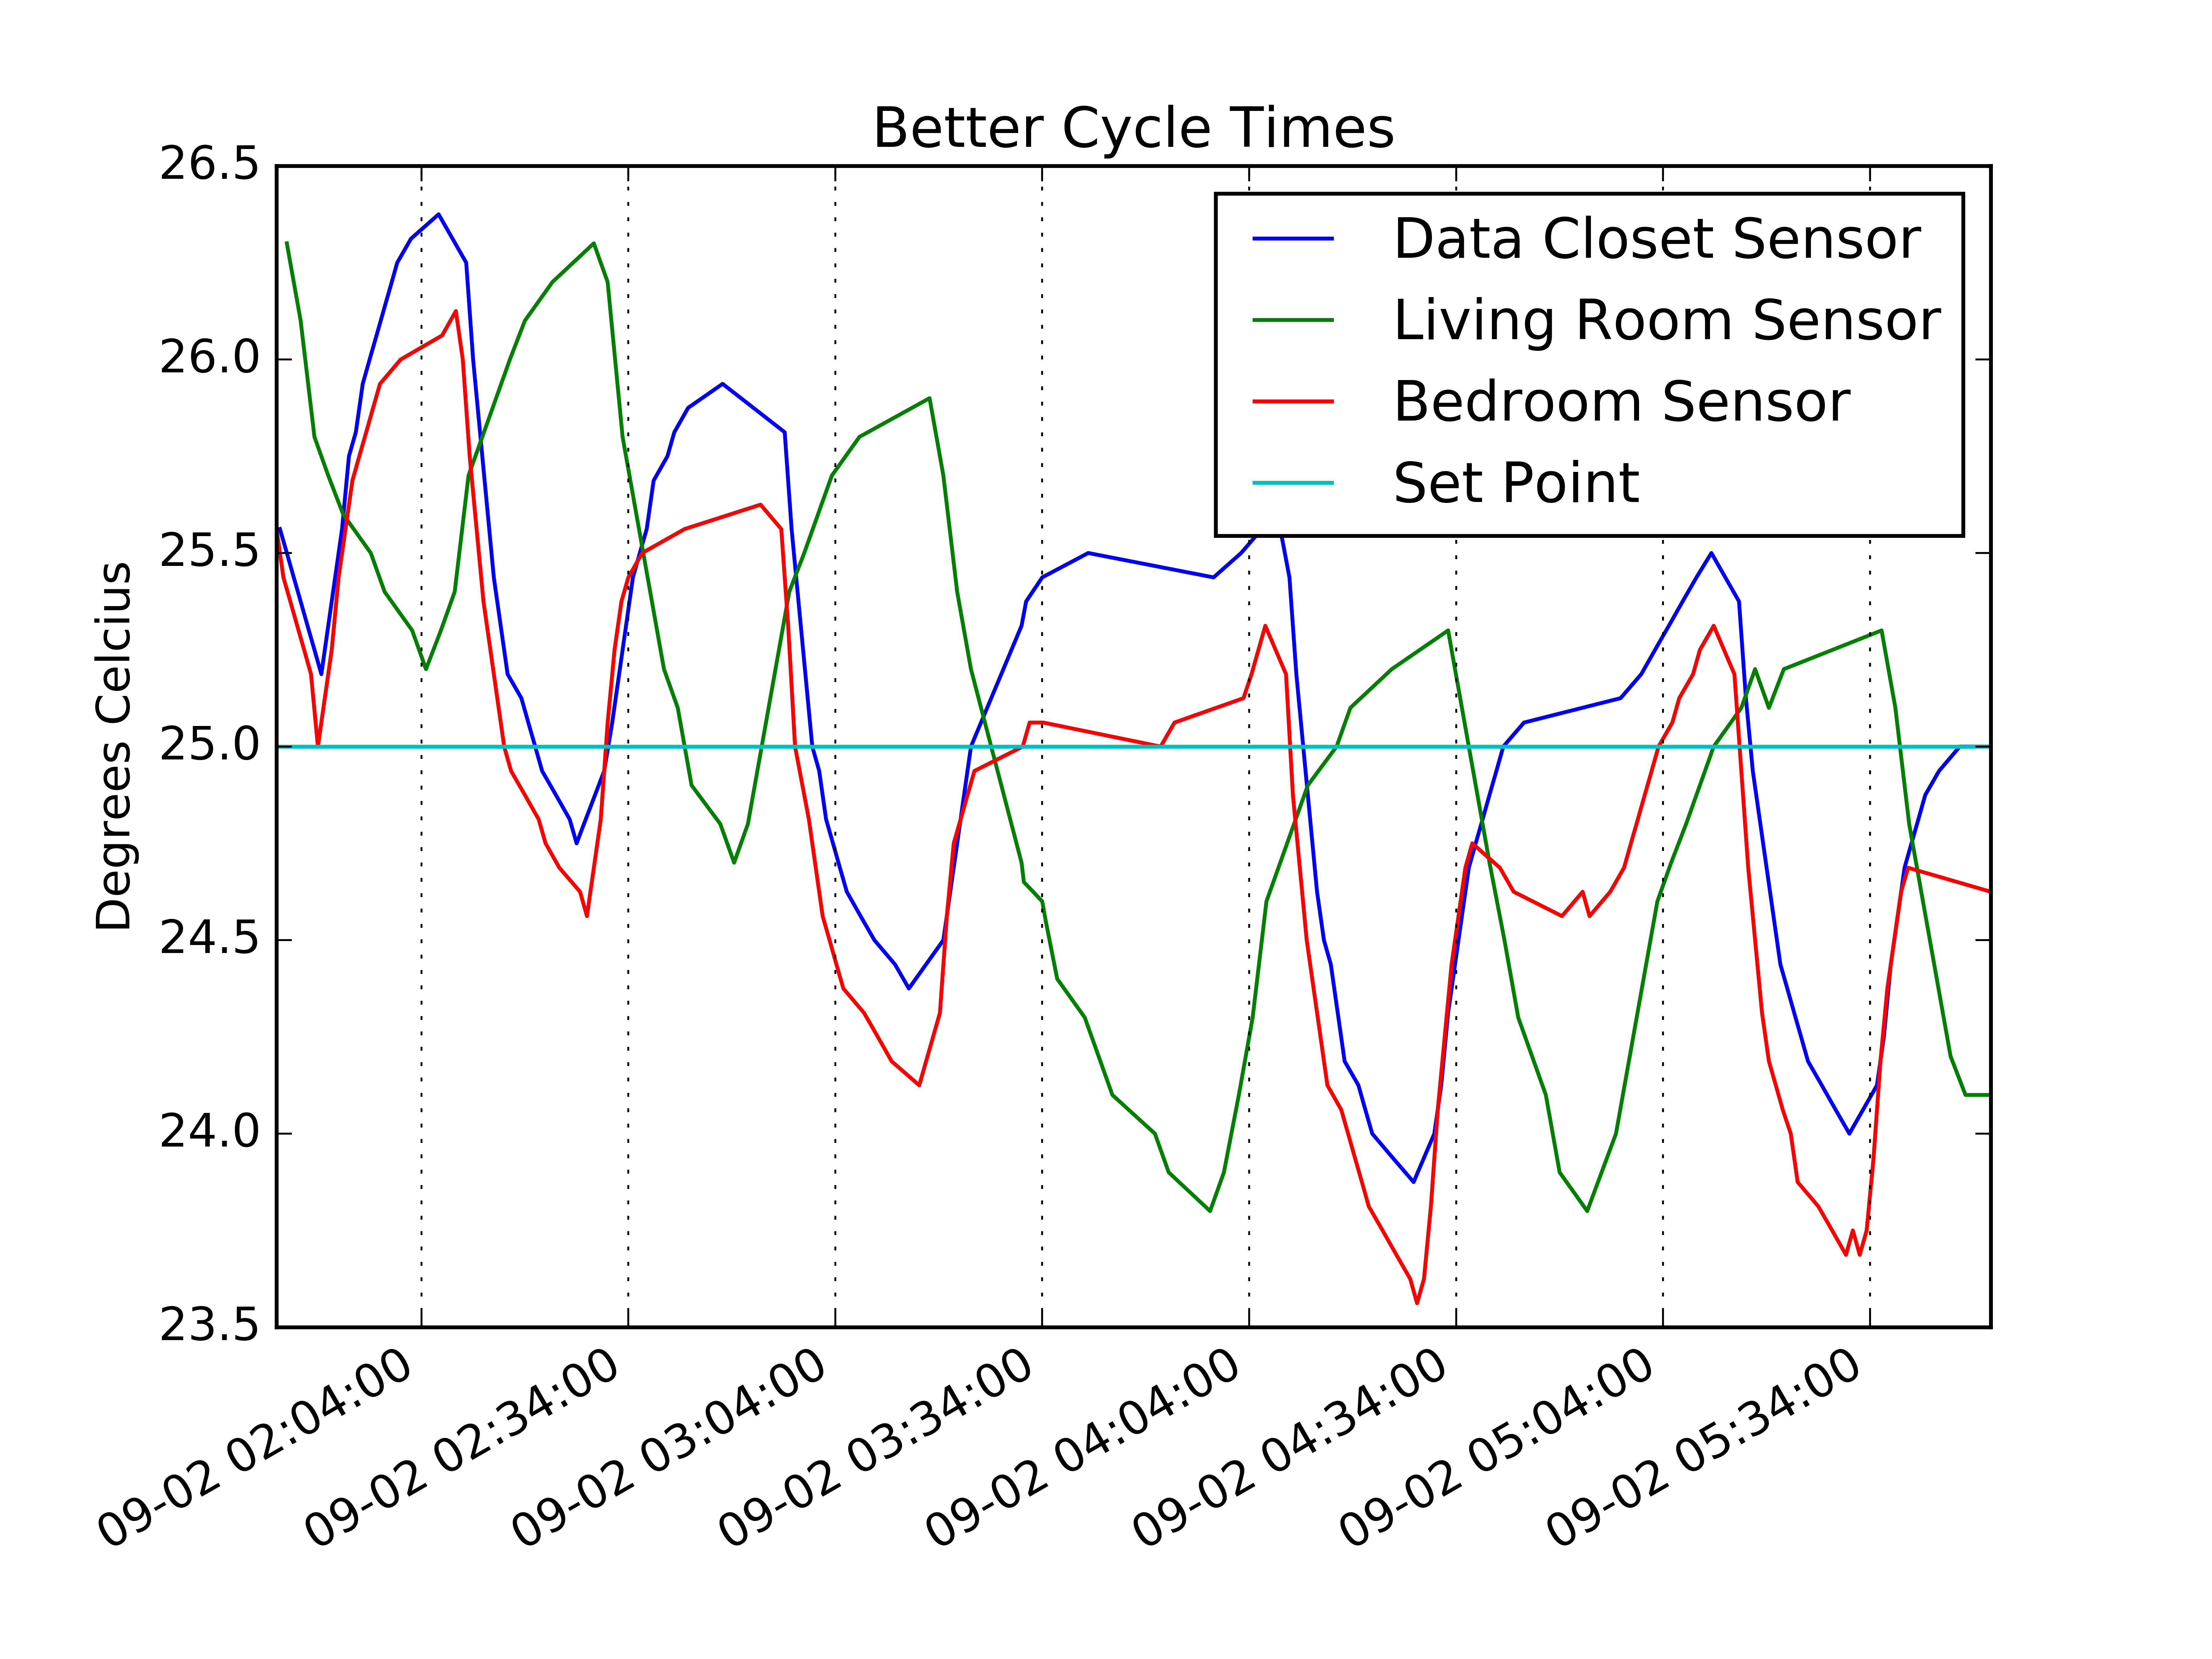
\includegraphics[height=.75\textheight]{long_cycle.png}
    \end{center}
    \begin{itemize}
        \item Bedroom on for 20 min. and off for 21 min.
        \item Living Room on for 17 min. off for 29 min.
    \end{itemize}
\end{frame}

\section{Automation}
\begin{frame}
\frametitle{Starting to Automate}
%    \begin{lstlisting}
      alias: Set Living Room AC to 30 C when asleep
      trigger:
        platform: time
        after: '12:30:00'
      condition:
        - condition: time
          before: '09:30:00'
      action:
        service: thermostat.set\_temperature
        entity\_id: thermostat.living\_room
        data:
          temperature: 28
%    \end{lstlisting}
\end{frame}

\subsection{Location based rules}
\begin{frame}
    \frametitle{Location Tracking}
    \begin{itemize}
        \item Start writing rules based on my location
        \item Set temperature higher when I'm not home
        \item Pre-cool
    \end{itemize}
\end{frame}

\begin{frame}
    \frametitle{Owntracks}
    \begin{columns}[T]
        \begin{column}{.48\textwidth}
            \begin{itemize}
                \item Open Source iOS and Android app for reporting location over MQTT
                \item Enables you to use either a private MQTT broker or public service
                \item Home assistant component to use the data
            \end{itemize}
        \end{column}
        \begin{column}{.48\textwidth}
            \centering
            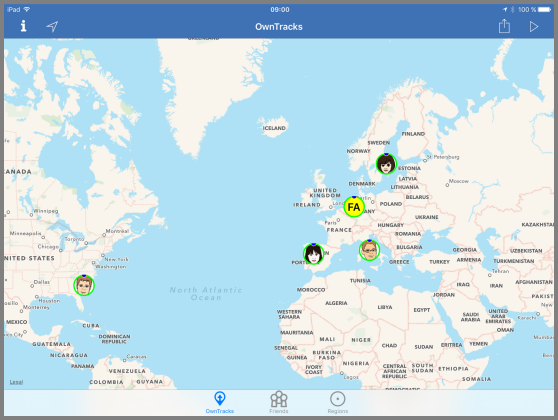
\includegraphics[width=.8\textwidth]{ipad-public-map.png}
        \end{column}
    \end{columns}
\end{frame}

\begin{frame}
    \frametitle{Location Based Automation Rules}
    alias: Set Living Room AC to 26 C when leaving starbucks route 9
    trigger:
      platform: state
      entity\_id: device\_tracker.myphone
      from: 'Starbucks Route 9'
    action:
      - delay:
          minutes: 5
      - service: climate.set\_temperature
        entity\_id: climate.living\_room
        data:
          temperature: 26
\end{frame}

\section{Conclusions}
\begin{frame}
    \frametitle{Future Work}
    \begin{itemize}
        \item More Sensors
        \item More automation
        \item Fix power usage collection
    \end{itemize}
\end{frame}

\section{More Information}
\begin{frame}
\frametitle{Where to get more information}
    \begin{itemize}
        \item Blog Post \href{http://blog.kortar.org/?p=319}{http://blog.kortar.org/?p=319}
        \item \href{https://home-assistant.io/}{https://home-assistant.io/}
        \item \href{https://github.com/mtreinish/dallasMQTT}{https://github.com/mtreinish/dallasMQTT}
        \item \href{http://owntracks.org/}{http://owntracks.org/}
    \end{itemize}
\end{frame}

\section{Questions}
\begin{frame}
\frametitle{Questions?}
\end{frame}

\end{document}
